\newpage
\section{8086 Microprocessor}
The 8086 microprocessor is an enhanced version of the 8085 microprocessor developed by Intel in 1978. It is a 16-bit microprocessor, with 20 address lines and 16 data lines to provide up to 1 MB of physical memory. 

    \begin{figure}[h]
        \begin{center}
            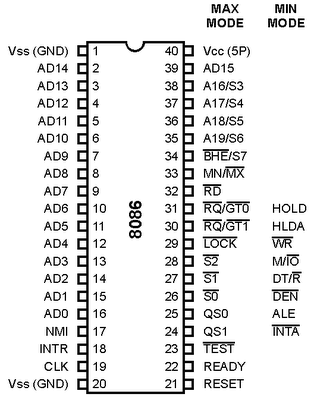
\includegraphics[width=0.35\textwidth]{figures/01_8086.png}
            \caption{8086 Microprocessor} \label{fig:8086}
        \end{center}
    \end{figure}

    \subsection{Features}
    The 8086 microprocessor is known for its significant advancements since its predecessors. The most prominent features include, but are not limited to:

    \begin{itemize}

        \item 6 bytes of cache memory for faster processing

        \item Pipelining stages: Fetch Stage and Execute Stage

        \item Instruction queue

        \item 256 vectored interrupts

        \item Maximum and minimum modes of operation, suitable for multiple and single processors respectively

    \end{itemize}

    \begin{figure}[h]
        \begin{center}
            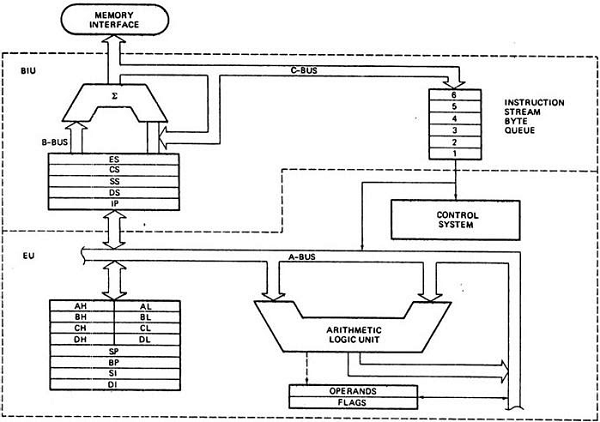
\includegraphics[width=0.5\textwidth]{figures/02_8086_architecture.jpg}
            \caption{Architecture of 8086} \label{fig:8086_architecture}
        \end{center}
    \end{figure}

    \subsection{Address and Data Buses}    

    \subsection{Control Bus}
